\section{A benchmark problem with analytical solution}


Let $\Omega=[0,1]^3$, $\Lambda=\{x=\tfrac{1}{2}\}\times \{y=\tfrac{1}{2}\} \times [0,1] $
and $\Sigma=[\tfrac{1}{4}, \tfrac{3}{4}]\times [\tfrac{1}{4}, \tfrac{3}{4}]\times [0, 1]$.
Finally we let $\DD$ be the cross section of the virtual interface $\Gamma=\partial \Sigma$.
As a benchmark for the two formulations we consider the following coupled problems
%
\begin{subequations}\label{benchmark}
\begin{align}
\label{benchm_3d}
-\Delta u=f \quad &\text{in $\Omega$}\\
\label{benchm_1d}
-d_{zz}^2 \ud =g \quad &\text{on $\Lambda$}\\
u=h \quad &\text{on $\partial \Omega$},
\end{align}
\end{subequations}
where for formulation \eqref{eq:problem1} the mix-dimensional coupling constraint reads
\begin{equation}
  \label{eq:couple_1}
\trace{u} - \ext{\ud} = q_1\quad\text{ on }\Gamma,
\end{equation}
while for \eqref{eq:problem2} we set
\begin{equation}
    \label{eq:couple_2}
\avrc{u} - \ud = q_2\quad\text{ on }\Lambda.
\end{equation}
%
In \eqref{benchmark}-\eqref{eq:couple_2} the right-hand sides shall be defined as 
\begin{eqnarray*}
  &f=8\pi ^2 \sin (2\pi x) \sin (2\pi y),\quad &g={\pi ^2}\sin \left({\pi z}\right),\quad h=\sin (2\pi x) \sin (2\pi y),\\
  &q_1=\sin (2\pi x) \sin (2\pi y) - \sin \left({\pi z}\right),\quad &q_2=-\sin \left({\pi z}\right).
\end{eqnarray*}

The exact solution of \eqref{benchmark}, regardless of the coupling constraint,
is given by
%
\begin{eqnarray}
\label{benchm_sol3d}
u=\sin (2\pi x) \sin (2\pi y)\\
\label{benchm_sol1d}
%\ud=1+\exp(-z).
\ud=\sin \left({\pi z}\right).
\end{eqnarray}
%
Let us notice that $\ud$ satisfies homogeneous Dirichlet conditions at the boundary of $\Lambda$.
Moreover, the solution \eqref{benchm_sol3d}-\eqref{benchm_sol1d} satisfies on $\Gamma$ the relation
\begin{equation}\label{benchm_flux}
L=\nabla u \cdot \textbf{n}_{\oplus}=d_z \ud n_{\oplus,z}=0,
\end{equation}
with $n_{\oplus,z}$ the $z-$component of the normal unit vector to $\Gamma$.

We prove that \eqref{benchmark} is solution of \eqref{eq:problem2} in the
simplified case in which the starting 3D-3D problem is
\begin{subequations}\label{eq:dirneu_simple}
\begin{align}
- \Delta \up  &= f  && \text{ in } \Omega_{\oplus},\\
- \Delta \uf &= g  && \text{ in } \Sigma,\\
-\nabla \uf \cdot \nn_{\ominus} &= -\nabla \up \cdot \nn_{\ominus}  && \text{ on } \Gamma,\\
\uf - \up &= q_i  && \text{ on }  \Gamma,\\
\up &= h && \text{ on } \partial \Omega.
\end{align}
\end{subequations}
instead of \eqref{eq:dirneu}. Therefore the reduced problem in \eqref{eq:problem1} and
\eqref{eq:problem2} become respectively
%
\begin{subequations}\label{eq:problem1_simple}
\begin{align}
\label{eq:problem1_simple_eq1}
&(\nabla u,\nabla v)_{L^2(\Omega)} + |{\cal D}|(d_s \ud,d_s \vd)_{L^2(\Lambda)} 
+ \langle \trace{v}  - \ext{\vd}, \lambda \rangle_\Gamma
\\
\nonumber
&\qquad\qquad= (f,v)_{L^2(\Omega)} + |{\cal D}| (\avrd{g},\vd)_{L^2(\Lambda)}
\quad \forall v \in H^1_0(\Omega), \ \vd \in H^1_0(\Lambda)
\\
\label{eq:problem1_simple_eq2}
&   \langle \trace{u} - \ext{\ud} , \mu \rangle_\Gamma =  \langle q_1 , \mu \rangle_\Gamma
\quad \forall \mu \in H^{-\frac12}(\Gamma)\,.
\end{align}
\end{subequations}
and
\begin{subequations}\label{eq:problem2_simple}
  \begin{align}
    \label{eq:problem2_simple_eq1}
&(\nabla u,\nabla v)_{L^2(\Omega)} + |{\cal D}|(d_s \ud,d_s \vd)_{L^2(\Lambda)} 
+ |{\partial \cal D}| \langle \avrc{v} - \vd, \ld \rangle_{H^{-\frac12}(\Lambda)} 
\\
\nonumber
&\qquad\qquad= (f,v)_{L^2(\Omega)} + |{\cal D}| (\avrd{g}, \vd)_{L^2(\Lambda)}
\quad \forall v \in H^1_0(\Omega), \ \vd \in H^1_0(\Lambda)
\\
\label{eq:problem2_simple_eq2}
&  |\partial {\cal D}| \langle \avrc{u} -  \ud, \md \rangle_{H^{-\frac12}(\Lambda)} =
|\partial {\cal D}| \langle \avrc{q_2}, \md \rangle_{H^{-\frac12}(\Lambda)}
\quad \forall \md \in H^{-\frac12}(\Lambda)\,.
\end{align}
\end{subequations}

Let us prove that \eqref{benchm_sol3d}-\eqref{benchm_sol1d} is solution of
\eqref{eq:problem2_simple}. Using the integration by part formula and homogeneous
boundary conditions on $\Omega$ and $\Lambda$, from \eqref{eq:problem2_simple_eq1} we have
\begin{align*}
&-(\Delta u, v)_{L^2(\Omega)} - |{\cal D}|(d^2_{ss} \ud, \vd)_{L^2(\Lambda)} 
+ |{\cal D}|\langle \avrc{v}  - \vd, \ld \rangle_\Lambda
\\
\nonumber
&\qquad\qquad= (f,v)_{L^2(\Omega)} + |{\cal D}| (\avrd{g},\vd)_{L^2(\Lambda)}
\quad \forall v \in H^1_0(\Omega), \vd \in H^1(\Lambda).
\\
\end{align*}
Since $\ld=\avrc{L}=0$ and \eqref{benchm_sol3d} satisfies \eqref{benchm_3d} and \eqref{benchm_sol1d}
satisfies \eqref{benchm_1d}, we have that
\begin{align*}
-(\Delta u, v)_{L^2(\Omega)} =  (f,v)_{L^2(\Omega)} \\
-|{\partial \cal D}|(d^2_{ss} \ud, \vd)_{L^2(\Lambda)}  = |{\cal D}| (\avrd{g},\vd)_{L^2(\Lambda)},
\end{align*}
Thus \eqref{benchm_sol3d}-\eqref{benchm_sol1d} satisfy \eqref{eq:problem2_simple_eq1}.
The fact that the solution satisfy \eqref{eq:problem2_simple_eq2} follows from \eqref{eq:couple_2}.

We can prove in a similar way that \eqref{benchm_sol3d}-\eqref{benchm_sol1d}, with $\lambda=0$
satisfy \eqref{eq:problem1_simple}. Note in particular that $q_1$ is such that
$\trace{u} - \ext{\ud} = q_1$ on $\Gamma$.

\subsection{Numerical experiments} Using the benchmark problem \eqref{benchmark}
we now investigate convergence properties of the two formulations. To this
end we consider a \emph{uniform} tessilation of $\mathcal{T}^{\Omega}_h$ of $\Omega$ consisting of
tetrahedra with diameter $h$. Further, the discretization shall be
geometrically \emph{conforming} to both $\Lambda$ and $\Gamma$ such that
the tessilations $\mathcal{T}^{\Gamma}_h$, $\mathcal{T}^{\Lambda}_h$ are made up
of facets and edges of $\mathcal{T}^{\Omega}_h$ respectively, cf. Figure \ref{fig:mesh}
for illustration.

\begin{figure}
  \begin{center}
    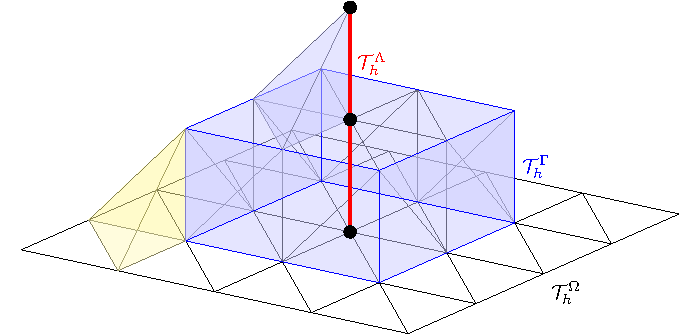
\includegraphics[width=0.5\textwidth]{./graphics/conform_mesh.pdf}
    \caption{$\Lambda$ and $\Gamma$ conforming discretization of $\Omega$
      used for \eqref{eq:problem1_simple} and \eqref{eq:problem2_simple}.
    }
    \label{fig:mesh}
  \end{center}
\end{figure}
  
Formulations \eqref{eq:problem1_simple} and \eqref{eq:problem2_simple} shall
be discretized using contiuous Lagrange element of order 1 ($P_1$) for all the spaces
involved. We recall that since we are investigating the conforming case, the tripplet
$P_1$-$P_1$-$P_1$ satisfies
the discrete inf-sup condition. The resulting linear systems are solved
using the minimal residual method (MinRes) with stopping criterion requiring the relative
preconditioned residual norm to be less than $10^{-12}$. As the preconditioner
we use the (approximate) Riesz mapping with respect to the inner products of
the spaces in which the two formulations were proved to be well posed.
In particular, the preconditioner for the Lagrange multiplier relies on
(the inverse of) the fractional Laplacian $-\Delta^{-1/2}$ on $\Gamma$ for
\eqref{eq:problem1_simple} and $\Lambda$ for \eqref{eq:problem2_simple}.
We remark that the size of the linear systems on the finest meshes considered
here prevents the use direct solvers. Therefore iterative solvers were necessary.
We plot the numerical solution of problem \eqref{eq:problem1_simple} and \eqref{eq:problem2_simple} in
Figure \ref{fig:sol_benchm1} and \ref{fig:sol_benchm2}, respectively. 

\begin{figure}
\centering
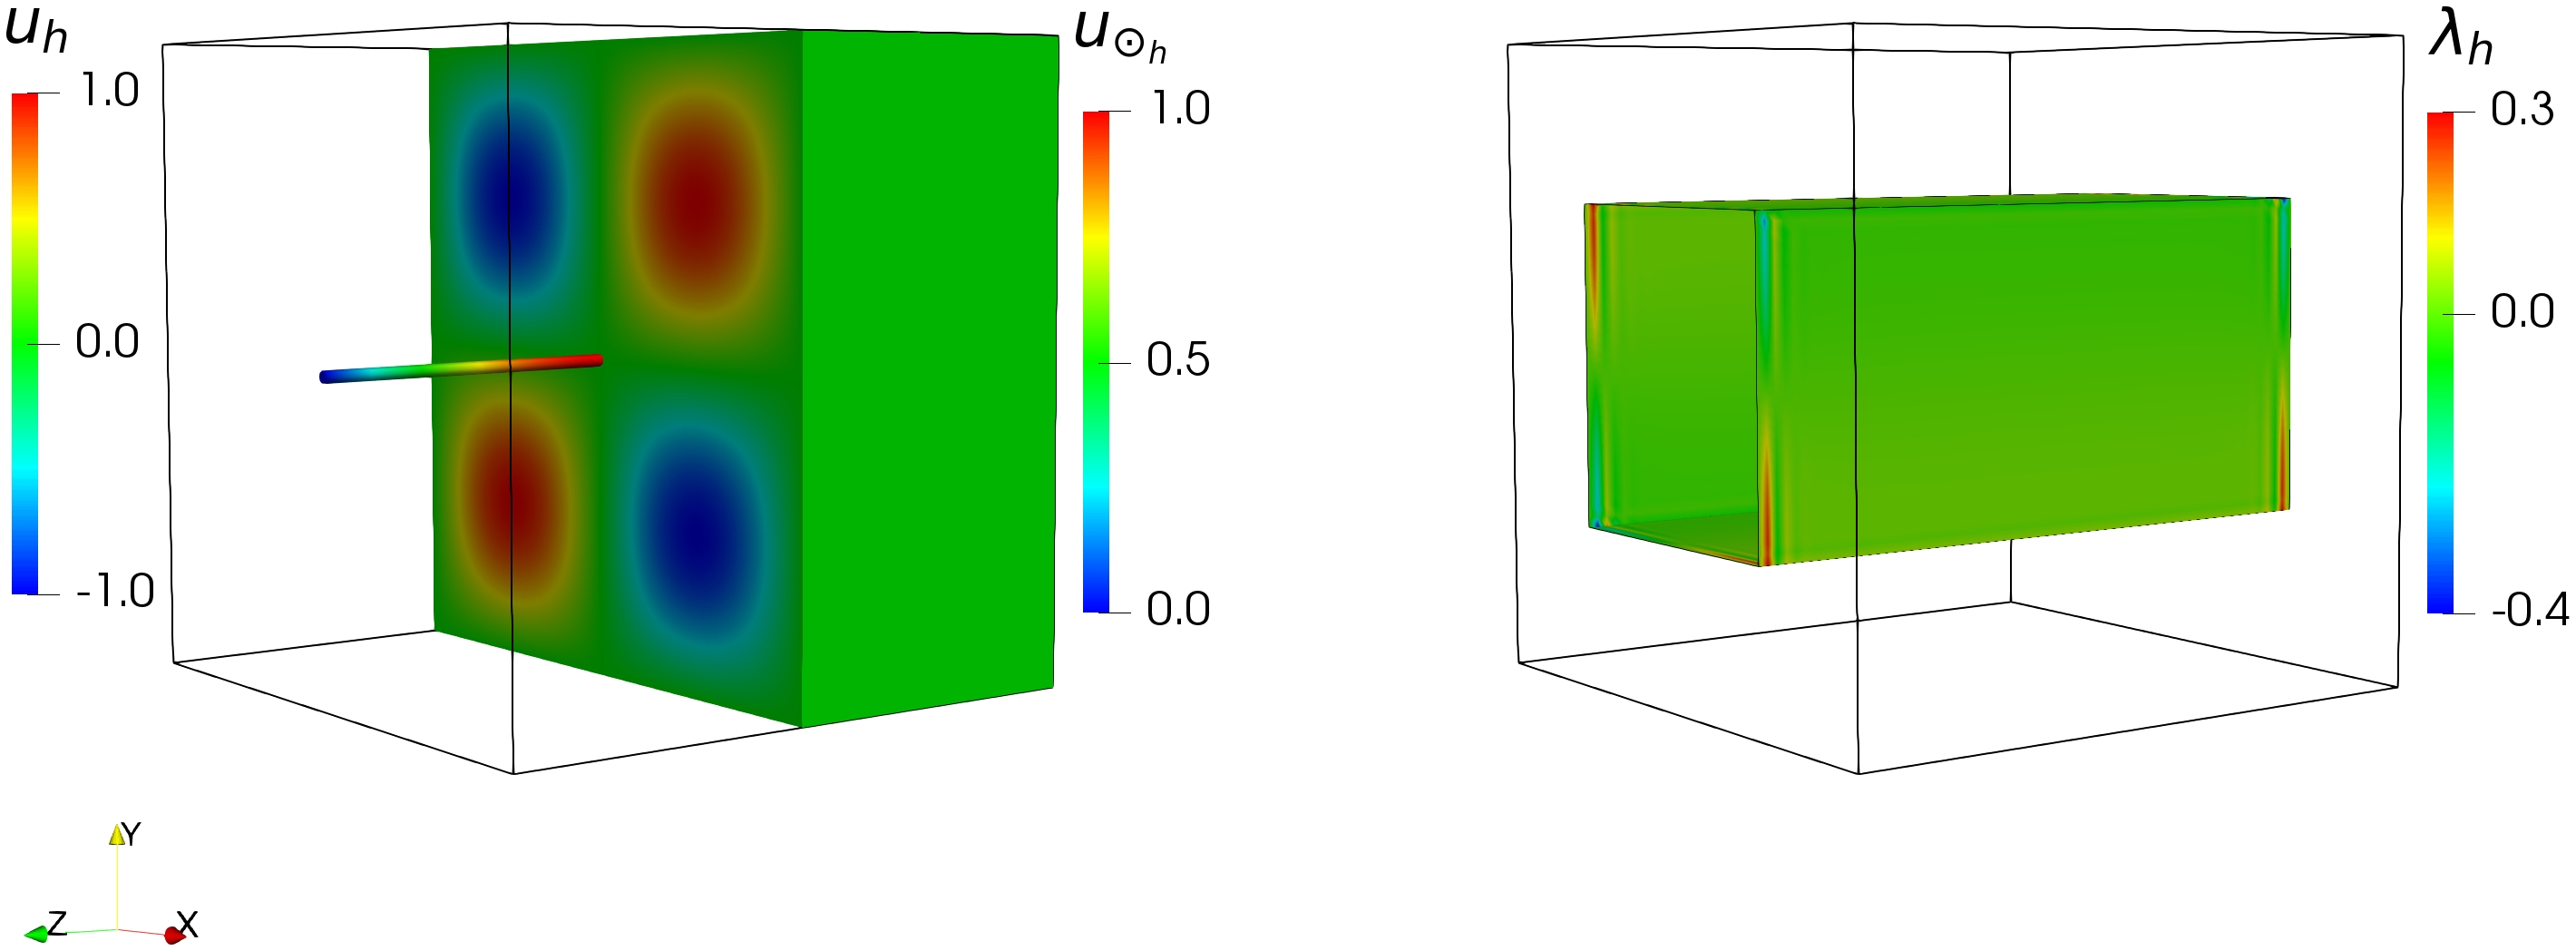
\includegraphics[width = 0.9\textwidth]{./graphics/mfs_LM2d}
\caption{Numerical solution of problem \eqref{eq:problem1_simple}: functions $u_h$ and $\udh$ on the left and the Lagrance multiplier $\lambda_h$ on the right.}\label{fig:sol_benchm1}
\end{figure}

\begin{figure}
\centering
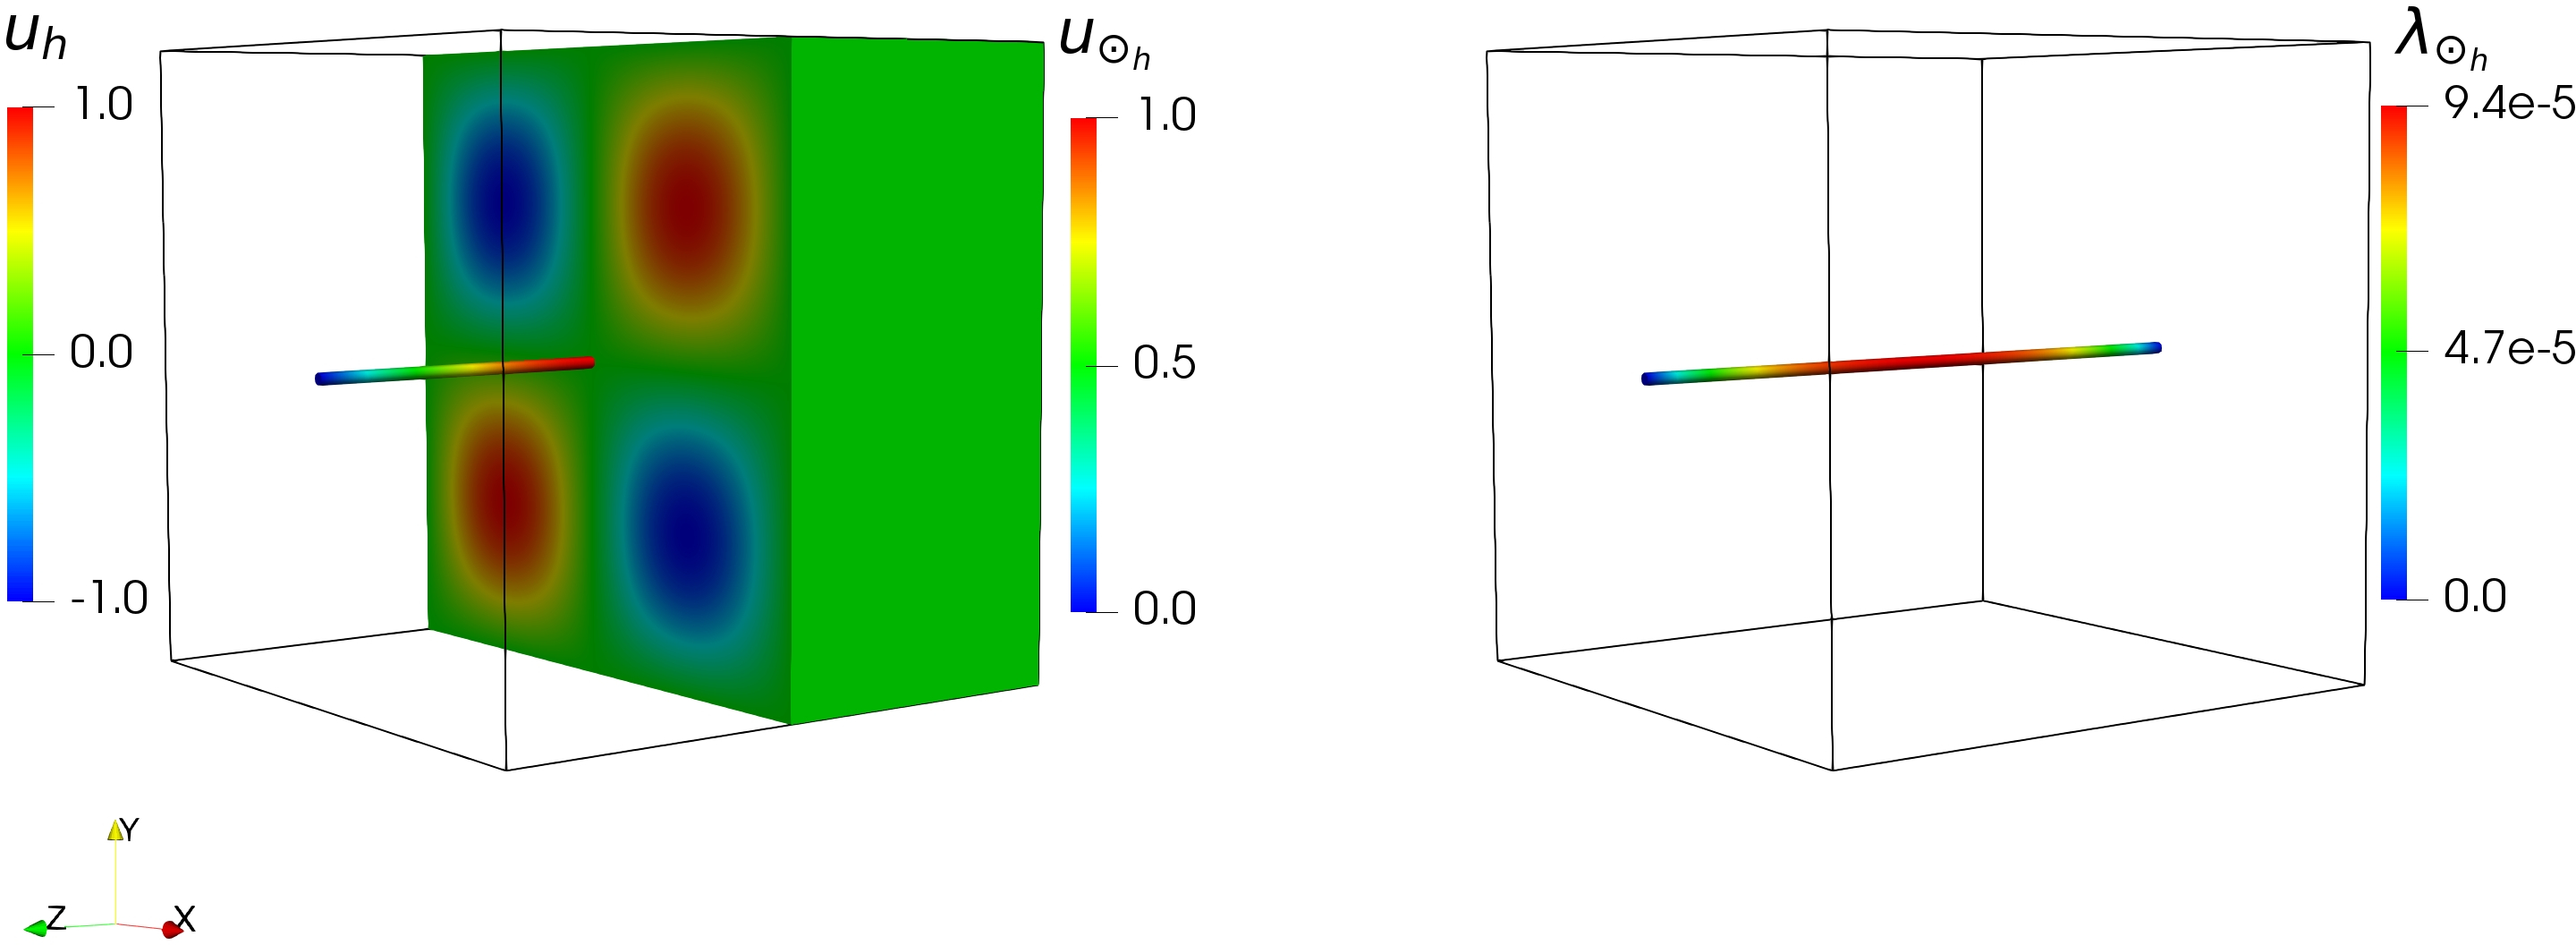
\includegraphics[width = 0.9\textwidth]{./graphics/mfs_LM1d}
\caption{Numerical solution of problem \eqref{eq:problem2_simple}: functions $u_h$ and $\udh$ on the left and the Lagrance multiplier ${\ld}_h$ on the right.}\label{fig:sol_benchm2}
\end{figure}

Considering uniform refinements of the initial mesh, Table \ref{tab:error_conform}
lists the errors of formulations \eqref{eq:problem1_simple} and \eqref{eq:problem2_simple}
on the benchmark problem. It can be seen the error in $u$ and $\ud$ in $H^1$ norm
converges linearly (as can be expected due to $P_1$ element discretization).
Moreover, the error of the Lagrange multiplier approximation in $H^{-1/2}$ norm
decreases quadratically. In the light of $P_1$ discretization this rate appears
superconvergent. We speculate that the result is due to the fact that the
exact solution is particularly simple, $L=0$. In case of the results for
\eqref{eq:problem1_simple} the rate can also be due to the fact that the
error is interpolated into the same finite element space as the approximation $L_h$.
We remark that for $u$ and $\ud$ the error is interpolated into FE space of piecewise
quadratic \emph{discontinous} functions. For \eqref{eq:problem2_simple} we
evaluate the fractional norm and interpolate the error using piecewise continuous
cubic functions. Evaluating the fractional norm in higher order spaces
for formulation with the multiplier space on $\Gamma$ is prohibitively costly. 

%
\begin{table}
  \scriptsize{
    \begin{minipage}{0.49\textwidth}
  \begin{center}
    \begin{tabular}{l|lll}
      \hline
    $h^{-1}$ & $\norm{u-u_h}_{1, \Omega}$ & $\norm{\ud-\udh}_{1, \Lambda}$ & $\norm{\lambda-\lambda_h}_{-1/2,\Gamma}$\\
      \hline
4  & 3.4E0(--) & 5.3E-1(--) & 2.9E0(--)\\
8  & 1.7E0(0.99) & 2.6E-1(1.06) & 6.1E-1(2.25)\\
16 & 8.7E-1(0.99) & 1.3E-1(1.02) & 1.4E-1(2.13)\\
32 & 4.4E-1(1.00) & 6.3E-2(1.00) & 3.4E-2(2.03)\\
64 & 2.2E-1(1.00) & 3.1E-2(1.00) & 8.6E-3(2.00)\\
\hline
  \end{tabular}
  \end{center}
  \end{minipage}
    }
    \vspace{5pt}
  \scriptsize{%(ii)
    \begin{minipage}{0.49\textwidth}
      \begin{center}
        \begin{tabular}{l|lll}
      \hline
    $h^{-1}$ & $\norm{u-u_h}_{1, \Omega}$ & $\norm{\ud-\udh}_{1, \Lambda}$ & $\norm{\ld-\ldh}_{-1/2, \Lambda}$\\
      \hline
4   & 3.1E0(--)    & 5.4E-1(--)   & 4.4E-2(--)   \\
8   & 1.7E0(0.87)  & 2.6E-1(1.06) & 1.1E-2(2.01) \\
16  & 8.6E-1(0.96) & 1.3E-1(1.02) & 2.7E-3(2.01) \\
32  & 4.4E-1(0.99) & 6.3E-2(1.00) & 6.7E-4(2.01) \\
64  & 2.2E-1(1.00) & 3.1E-2(1.00) & 1.7E-4(2.01) \\
128 & 1.1E-1(1.00) & 1.6E-2(1.00) & 4.1E-5(2.01) \\
\hline
  \end{tabular}
  \end{center}
  \end{minipage}
  }
  \caption{Error convergence of \eqref{eq:problem1_simple} and \eqref{eq:problem2_simple}
    on a benchmark problem \eqref{benchmark}. Continuous linear Lagrange
    elements are used.
  }
  \label{tab:error_conform}
\end{table}

In Table \ref{tab:error_conform} one can observe that the two formulations
yield practically identical approximations of $u$ and $\ud$. However, the solution
cost of the two approaches differs. In Table \ref{tab:cost} we summarize the
size of the linear systems solved at each level of refinement and the time
for the iterative solver to converge. Let us first note that the proposed
preconditioners seem robust with respect to discretization parameter as
the iteration counts are clearly bounded. We then see that the solution
time for \eqref{eq:problem1_simple} is about 2 times longer compared to
\eqref{eq:problem2_simple}. This is in addition to the higher setup costs
of the preconditioner which in our implementation involve solving an eigenvalue
problem for the fractional Laplacian. Therefore it is advantageous to keep
the multiplier space as small as possible. We remark that the missing
results for \eqref{eq:problem1_simple} in Table \ref{tab:cost} and \ref{tab:error_conform}
are due to the memory limitations which we encounter when solving the eigenvalue problem
for the Laplacian, which for finest mesh involves cca 32 thousand eigenvalues.
%
\begin{table}
  \scriptsize{
  \begin{center}
    \begin{tabular}{l|ll|lll|lll}
      \hline
      $h^{-1}$ & $\dim{X^1_{h, 0}(\Omega)}$ & $\dim{X^1_{h, 0}(\Lambda)}$ & $\dim{Q_h(\Gamma)}$ & $\#$ & $T\left[s\right]$ & $\dim{Q_h(\Lambda)}$ & $\#$ & $T\left[s\right]$\\
      \hline
4   &125     &5   &40    &27 &0.03  &5   &9  &0.01\\
8   &729     &9   &144   &55 &0.10  &9   &19 &0.02\\
16  &4913    &17  &544   &62 &0.25  &17  &36 &0.14\\
32  &35937   &33  &2112  &64 &1.97  &33  &42 &1.08\\
64  &274625  &65  &8320  &64 &18.01 &65  &36 &8.24\\
128 &2146947 &129 &--    &-- &--    &129 &31 &61.37\\
\hline
    \end{tabular}
    \end{center}
    }
  \caption{Cost comparison of the two formulations. Number of MinRes iterations
    is denoted by $\#$. Time till convergence of the iterative solver (excluding the setup) is shown
    as $T$.
  }
\label{tab:cost}
\end{table}

%\begin{remark}
%Let us notice that the 3D solution \eqref{benchm_sol3d} is such that $\avrc{u}=0$. Therefore in \eqref{benchmark} it is like we are solving two separated problems, one in $\Omega$ and the other on $\Lambda$.
%\end{remark}
%\begin{remark}
%It would be interesting to make a comparison between the solution of the fully coupled 3D-3D problem \eqref{eq:dirneu} (also in the simplified case of type \eqref{eq:dirneu_simple}) and the solution of the reduced problems \eqref{eq:problem1} and \eqref{eq:problem2}. 
%Therefore, we could set the values of the data of the problem such that the reduced formulation becomes non-trivial and fully coupled.
%Then, we will solve both the original and reduced problem to observe the differences in the solutions and the values of the Lagrange multiplier.
%\end{remark}
